
Write a function that accepts a matrix $A$, a vector $\b$, and an initial guess $\x_0$, a maximum number of iterations $k$ defaulting to $100$, and a stopping tolerance \li{tol} that defaults to $10^{-8}$.
Use Algorithm \ref{alg:gmres} to approximate the solution to $A\x=\b$ using the GMRES algorithm.
Return the approximate solution and the residual at the approximate solution.

You may assume that $A$ and $\b$ only have real entries.
Use \li{scipy.linalg.lstsq()} to solve the least squares problem.
Be sure to read the documentation so that you understand what the function returns.

Compare your function to the following code.
\begin{lstlisting}
>>> A = np.array([[1,0,0],[0,2,0],[0,0,3]])
>>> b = np.array([1, 4, 6])
>>> x0 = np.zeros(b.size)
>>> gmres(A, b, x0, k=100, tol=1e-8)
(array([ 1.,  2.,  2.]), 7.174555448775421e-16)
\end{lstlisting}
\label{prob:MyGMRES}

\label{prob:plot_gmres}
Add a keyword argument \li{plot} defaulting to \li{False} to your function from Problem \ref{prob:MyGMRES}.
If \li{plot=True}, keep track of the residuals at each step of the algorithm.
At the end of the iteration, before returning the approximate solution and its residual error, create a figure with two subplots.
\begin{enumerate}
\item Make a scatter plot of the eigenvalues of $A$ on the complex plane.
\item Plot the residuals versus the iteration counts using a log scale on the $y$-axis\\(use \li{ax.semilogy()}).
\end{enumerate}

\label{prob:make_plots}
Use your function from Problem \ref{prob:plot_gmres} to investigate how the convergence of GMRES relates to the eigenvalues of a matrix as follows.
Define an $m\times m$ matrix
\[A_n = nI+P,\]
 where $I$ is the identity matrix and $P$ is an $m \times m$ matrix with entries taken from a random normal distribution with mean 0 and standard deviation $1/(2\sqrt{m})$.
 Call your function from Problem \ref{prob:plot_gmres} on $A_n$ for $n=-4,-2,0,2,4$.
 Use $m=200$, let $\b$ be an array of all ones, and let $\x_0 = \0$.

Use \li{np.random.normal()} to create the matrix $P$.
When analyzing your results, pay special attention to the clustering of the eigenvalues in relation to the origin.
Compare your results with $n=2$, $m=200$ to Figure \ref{fig:plot_gmres}.

Ideas for this problem were taken from Example 35.1 on p. 271 of \cite{Trefethen1997}.

\begin{figure}[H] % Convergence of GMRES.
\captionsetup[subfigure]{justification=centering}
\centering
\begin{subfigure}{.49\textwidth}
    \centering
    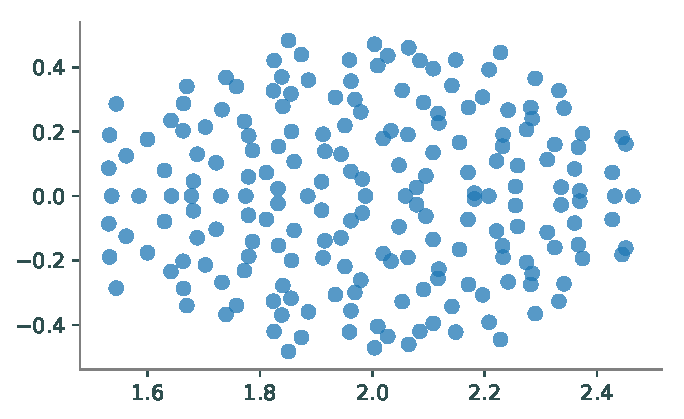
\includegraphics[width=\textwidth]{figures/scatter_gmres.pdf}
\end{subfigure}
%
\begin{subfigure}{.49\textwidth}
    \centering
    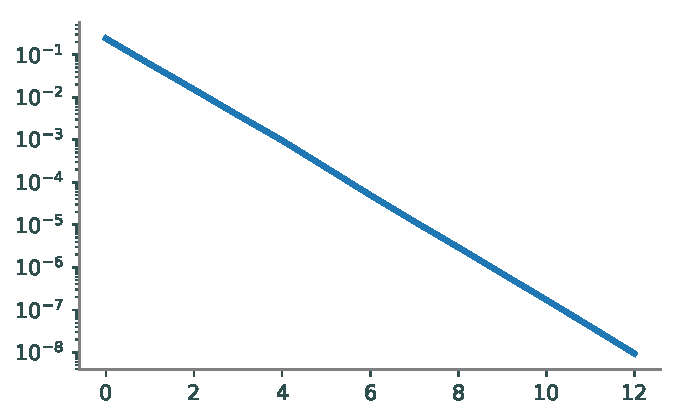
\includegraphics[width=\textwidth]{figures/gmres_convergence.pdf}
\end{subfigure}
\caption{On the left, the eigenvalues of the matrix $A_2$ defined in Problem \ref{prob:make_plots}.
On the right, the rapid convergence of the GMRES algorithm on $A_2$ with starting vector $\b = (1, 1, \ldots, 1)$.}
\label{fig:plot_gmres}
\end{figure}

 \label{prob:GMRES2}
 (Optional) Modify MyGMRES to incorporate these optimizations, and call this program MyGMRES1.
 Run both programs on a series of five random $100\times 100$ matrices and compare the time each requires.
 Are the gains substantial?
 Try it again matrices of size $1000\times 1000$ or larger, and see how substantial the difference becomes.
 Try the same thing using the techniques of the next section.
 Explain why the difference in performance is less dramatic this time.
 
Write a function that implements GMRES with restarts as follows.
\begin{enumerate}
\item Perform the GMRES algorithm for a maximum of k iterations.
\item If the desired tolerance was reached, terminate the algorithm.
If not, repeat step 1 using $x_k$ from the previous GMRES algorithm as a new initial guess $x_0$.
\item Repeat step 2 until the desired tolerance has been obtained or until a given maximum number of restarts has been reached.
\end{enumerate}
Your function should accept all of the same inputs as the function you wrote in Problem 1 with the exception of $k$, which will now denote the number of iterations before restart (defaults to $5$), and an additional parameter \li{restarts} which denotes the maximum number of restarts before termination (defaults to $50$).
\label{prob:GMRESk}

Plot the runtimes of your implementations of GMRES from Problems 1 and 4 and \li{scipy.sparse.linalg.gmres()} use the default tolerance and \li{restart=1000} with different matrices.
Use the $m \times m$ matrix $P$ with $m=25,50,\dots 200$ and with entries taken from a random normal distribution with mean 0 and standard deviation $1/(2\sqrt{m})$.
Use a vector of ones for $\b$ and a vector of zeros for $\x_0$.
Use a single figure for all plots, plot the runtime on the $y$-axis and $m$ on the $x$-axis.

Using the function \li{finite_difference()} from your iterative solvers lab, modify the \li{hot_plate()} function to use the GMRES algorithm instead of the SOR method.
Do you see any differences in speed?
Can you solve larger systems with GMRES?
Try the different versions of the GMRES algorithm that we have discussed, what differences do you see?
